
\documentclass[conference]{IEEEtran}

\IEEEoverridecommandlockouts
\usepackage{graphicx}

\usepackage[bitstream-charter]{mathdesign}
\usepackage[utf8]{inputenc}
\usepackage[T1]{fontenc}

\usepackage{amsmath, graphicx, setspace}

\usepackage[lofdepth,lotdepth]{subfig}
\usepackage[justification=centering, labelsep=space, figurewithin=none, tablewithin=none, labelfont=bf]{caption}
\usepackage{multirow}
\usepackage{array}

\hyphenchar\font=-1
\sloppy


\begin{document}

\title{BAŞLIK - Özetçe Hariç Tüm Doküman İngilizce Olmalıdır}


\author{
    \IEEEauthorblockN{Ahmet Elbir, Sercan Aygün}
    \IEEEauthorblockA{  Bilgisayar Mühendisliği Bölümü\\
                        Yıldız Teknik Üniversitesi, 34220 Istanbul,  Türkiye\\
                        \{aelbir, sercan\}@yildiz.edu.tr }
}

\maketitle

\begin{ozet}
Bu belge, SİU 2017 bildirisi hazırlamanız için bir taslak içermektedir. Bu sebeple lütfen taslaktaki başlık, özet ve diğer format stillerini kullanınız.  \textit{*Dikkat:  Bildiri Başlığında ve Özetlerde Sembol, Özel ve Matematiksel Karakterler kullanmayınız.}
%\boldmath
\end{ozet}
\begin{IEEEanahtar}
doküman biçimi, stil, anahtar kelimeler.
\end{IEEEanahtar}

\begin{abstract}
This electronic document is a “live” template and already defines the components of your paper [title, text, heads, etc.] in its style sheet.  \textit{*CRITICAL:  Do Not Use Symbols, Special Characters, or Math in Paper Title or Abstract.}
%\boldmath
\end{abstract}
\begin{IEEEkeywords}
component, formatting, style, styling, insert (key words).
\end{IEEEkeywords}


\section{Introduction}

Bu taslak, YTÜ Bilgisayar Mühendisliğinin Bilgisayar Projesi için teslim edilmesi gereken ara makale bildiri yazımı için önerdiği Latex taslağıdır. IEEE konferanslarında kullanılan taslak baz alımıştır. Kenar boşlukları, sütun genişlikleri, satır aralıkları ve stiller taslağın içine gömülüdür.  Taslağa bağlı kalmaya dikkat ediniz.\cite{WinNT}

\section{Kullanım}

\subsection{Taslak Seçmek}

Doğru taslağı (bu taslağı) kullandığınızdan emin olunuz.\cite{van2007experimental}

\subsection{Taslağın Formatına Bağlı Kalmak}

Taslağın formatını değiştirmeyiniz. \cite{guo2004learning}


\section{Sayfa Düzeni ve Biçim}

Lorem ipsum dolor sit amet, consectetur adipiscing elit. Nunc dui ex, varius a mattis sed, vestibulum varius ante. Aliquam maximus ut nisi quis efficitur. Maecenas laoreet nisl vitae tempor aliquam. Donec ac odio suscipit, suscipit magna vitae, pharetra sapien. Cras arcu libero, suscipit ut massa sit amet, tempus euismod augue. Cras eu ligula id nulla luctus facilisis ultrices sit amet lorem. Praesent placerat, lorem eget pharetra dictum, arcu est pharetra ante, vel suscipit mi odio nec sapien. Morbi vehicula elit lacus, sit amet tristique nisi interdum non. Cras convallis neque dui, ut aliquet nulla tempor elementum. Fusce sagittis urna ac mauris mattis condimentum.\cite{knauff2014efficiency}

Vivamus efficitur a purus eu egestas. Donec feugiat facilisis mauris, at gravida turpis. Mauris quis pellentesque est. Duis in quam sollicitudin massa facilisis fringilla. Proin pulvinar, justo sit amet hendrerit sollicitudin, massa quam euismod felis, porta cursus est tortor nec elit. In mollis nunc eget massa bibendum, vel sagittis enim placerat. Sed luctus porta felis, a faucibus nisi placerat a. Duis velit libero, gravida sed iaculis sodales, consectetur eget metus. Nulla vel magna purus. Sed ligula magna, dignissim sed convallis id, sodales vel libero.

\subsection{Kısaltmalar}

Kısaltmaları yazı içinde ilk defa kullanıldıklarında tanımlayınız. Başlıklarda kısaltma kullanmayınız. IEEE, SI, CGS vb. gibi çok bilinmiş kısaltmaları tanımlamanıza gerek yoktur.

\subsection{Birimler}

\begin{itemize}
\item SI veya CGS ölçü birimlerini kullanınız. (SI ölçü birimi tavsiye edilir.)
\item Yazı içinde farklı ölçü birimleri kullanmayınız. İngiliz ölçü birimlerini birinci birim olarak kullanmaktan kaçınınız. Ancak çok gerekli ise parantez içerisinde ikinci birim olarak gösteriniz.
\item Ölçü birimlerini yazarken tutarlılık sağlayınız. Örneğin “Wb/m2” veya “webers per square meter” kullanınız, “webers/m2” kullanmayınız.
\item Küsuratlı sayı kullanırken “.25” yerine “0.25” kullanınız.
\end{itemize}

\subsection{Denklemler}

Denklemler taslaktaki formata istisnadır. Denklemler asağıdaki örneğe benzemelidir.

\begin{equation}
\lim_{x \to \infty} \exp(-x) = 0
\end{equation}

Denklem merkezde olmalıdır. Denklemdeki sembolleri tanımladığınızdan emin olunuz. Denklemden bahsederken “(1)” kullanınız. Cümle başında “Denklem (1)” kullanabilirsiniz.

\subsection{Sayfa Sayısı}

Hazırlanacak bildiri, kaynaklar dahil, en fazla dört sayfa olmalıdır.

\subsection{Kaynak Formatı}

Bildiride kullanılan kaynaklar “Kaynaklar” bölümünde IEEE kaynak gösterim formatı kullanılarak listelenmelidir. Örnek bir “Kaynaklar” bölümü bu taslağın sonunda gösterilmiştir. 

\section{Taslağı Kullanmak}

\subsection{Yazarlar}

Lorem ipsum dolor sit amet, consectetur adipiscing elit. Nunc dui ex, varius a mattis sed, vestibulum varius ante. Aliquam maximus ut nisi quis efficitur. Maecenas laoreet nisl vitae tempor aliquam. Donec ac odio suscipit, suscipit magna vitae, pharetra sapien. Cras arcu libero, suscipit ut massa sit amet, tempus euismod augue. Cras eu ligula id nulla luctus facilisis ultrices sit amet lorem. Praesent placerat, lorem eget pharetra dictum, arcu est pharetra ante, vel suscipit mi odio nec sapien. Morbi vehicula elit lacus, sit amet tristique nisi interdum non. Cras convallis neque dui, ut aliquet nulla tempor elementum. Fusce sagittis urna ac mauris mattis condimentum.

Vivamus efficitur a purus eu egestas. Donec feugiat facilisis mauris, at gravida turpis. Mauris quis pellentesque est. Duis in quam sollicitudin massa facilisis fringilla. Proin pulvinar, justo sit amet hendrerit sollicitudin, massa quam euismod felis, porta cursus est tortor nec elit. In mollis nunc eget massa bibendum, vel sagittis enim placerat. Sed luctus porta felis, a faucibus nisi placerat a. Duis velit libero, gravida sed iaculis sodales, consectetur eget metus. Nulla vel magna purus. Sed ligula magna, dignissim sed convallis id, sodales vel libero.

\subsection{Başlıklar}

Lorem ipsum dolor sit amet, consectetur adipiscing elit. Nunc dui ex, varius a mattis sed, vestibulum varius ante. Aliquam maximus ut nisi quis efficitur. Maecenas laoreet nisl vitae tempor aliquam. Donec ac odio suscipit, suscipit magna vitae, pharetra sapien. Cras arcu libero, suscipit ut massa sit amet, tempus euismod augue. Cras eu ligula id nulla luctus facilisis ultrices sit amet lorem. Praesent placerat, lorem eget pharetra dictum, arcu est pharetra ante, vel suscipit mi odio nec sapien. Morbi vehicula elit lacus, sit amet tristique nisi interdum non. Cras convallis neque dui, ut aliquet nulla tempor elementum. Fusce sagittis urna ac mauris mattis condimentum.

Vivamus efficitur a purus eu egestas. Donec feugiat facilisis mauris, at gravida turpis. Mauris quis pellentesque est. Duis in quam sollicitudin massa facilisis fringilla. Proin pulvinar, justo sit amet hendrerit sollicitudin, massa quam euismod felis, porta cursus est tortor nec elit. In mollis nunc eget massa bibendum, vel sagittis enim placerat. Sed luctus porta felis, a faucibus nisi placerat a. Duis velit libero, gravida sed iaculis sodales, consectetur eget metus. Nulla vel magna purus. Sed ligula magna, dignissim sed convallis id, sodales vel libero.

\subsection{Şekil ve Tablolar}

\subsubsection{Şekil ve tabloların yerleştirilmeleri} 
Lorem ipsum dolor sit amet, consectetur adipiscing elit. Nunc dui ex, varius a mattis sed, vestibulum varius ante. Aliquam maximus ut nisi quis efficitur. Maecenas laoreet nisl vitae tempor aliquam. Donec ac odio suscipit, suscipit magna vitae, pharetra sapien. Cras arcu libero, suscipit ut massa sit amet, tempus euismod augue. Cras eu ligula id nulla luctus facilisis ultrices sit amet lorem. Praesent placerat, lorem eget pharetra dictum, arcu est pharetra ante, vel suscipit mi odio nec sapien. Morbi vehicula elit lacus, sit amet tristique nisi interdum non. Cras convallis neque dui, ut aliquet nulla tempor elementum. Fusce sagittis urna ac mauris mattis condimentum.

Vivamus efficitur a purus eu egestas. Donec feugiat facilisis mauris, at gravida turpis. Mauris quis pellentesque est. Duis in quam sollicitudin massa facilisis fringilla. Proin pulvinar, justo sit amet hendrerit sollicitudin, massa quam euismod felis, porta cursus est tortor nec elit. In mollis nunc eget massa bibendum, vel sagittis enim placerat. Sed luctus porta felis, a faucibus nisi placerat a. Duis velit libero, gravida sed iaculis sodales, consectetur eget metus. Nulla vel magna purus. Sed ligula magna, dignissim sed convallis id, sodales vel libero.

\subsubsection{Aksis tanımlamaları} 
Lorem ipsum dolor sit amet, consectetur adipiscing elit. Nunc dui ex, varius a mattis sed, vestibulum varius ante. Aliquam maximus ut nisi quis efficitur. Maecenas laoreet nisl vitae tempor aliquam. Donec ac odio suscipit, suscipit magna vitae, pharetra sapien. Cras arcu libero, suscipit ut massa sit amet, tempus euismod augue. Cras eu ligula id nulla luctus facilisis ultrices sit amet lorem. Praesent placerat, lorem eget pharetra dictum, arcu est pharetra ante, vel suscipit mi odio nec sapien. Morbi vehicula elit lacus, sit amet tristique nisi interdum non. Cras convallis neque dui, ut aliquet nulla tempor elementum. Fusce sagittis urna ac mauris mattis condimentum.

Vivamus efficitur a purus eu egestas. Donec feugiat facilisis mauris, at gravida turpis. Mauris quis pellentesque est. Duis in quam sollicitudin massa facilisis fringilla. Proin pulvinar, justo sit amet hendrerit sollicitudin, massa quam euismod felis, porta cursus est tortor nec elit. In mollis nunc eget massa bibendum, vel sagittis enim placerat. Sed luctus porta felis, a faucibus nisi placerat a. Duis velit libero, gravida sed iaculis sodales, consectetur eget metus. Nulla vel magna purus. Sed ligula magna, dignissim sed convallis id, sodales vel libero.

\begin{table}[!htbp]
  \centering
  \caption{\textsc{Örnek Tablo}}
  \label{tablo1}
        \begin{tabular}{|c|c|c|c|}
        \hline
        \multirow{3}{*}{\textbf{\begin{tabular}[c]{@{}c@{}}Tablo \\ Başlığı\end{tabular}}} & \multicolumn{3}{c|}{\textbf{Tablo sütun başlığı}} \\ \cline{2-4} 
         & \begin{tabular}[c]{@{}c@{}}Tablo sütun \\ ara başlığı\end{tabular} & Ara başlık & Ara başlık \\ \cline{2-4} 
         &  &  &  \\ \hline
        \end{tabular}
\end{table}

Lorem ipsum dolor sit amet, consectetur adipiscing elit. Nunc dui ex, varius a mattis sed, vestibulum varius ante. Aliquam maximus ut nisi quis efficitur. Maecenas laoreet nisl vitae tempor aliquam. Donec ac odio suscipit, suscipit magna vitae, pharetra sapien. Cras arcu libero, suscipit ut massa sit amet, tempus euismod augue. Cras eu ligula id nulla luctus facilisis ultrices sit amet lorem. Praesent placerat, lorem eget pharetra dictum, arcu est pharetra ante, vel suscipit mi odio nec sapien. Morbi vehicula elit lacus, sit amet tristique nisi interdum non. Cras convallis neque dui, ut aliquet nulla tempor elementum. Fusce sagittis urna ac mauris mattis condimentum.

Vivamus efficitur a purus eu egestas. Donec feugiat facilisis mauris, at gravida turpis. Mauris quis pellentesque est. Duis in quam sollicitudin massa facilisis fringilla. Proin pulvinar, justo sit amet hendrerit sollicitudin, massa quam euismod felis, porta cursus est tortor nec elit. In mollis nunc eget massa bibendum, vel sagittis enim placerat. Sed luctus porta felis, a faucibus nisi placerat a. Duis velit libero, gravida sed iaculis sodales, consectetur eget metus. Nulla vel magna purus. Sed ligula magna, dignissim sed convallis id, sodales vel libero.

\begin{figure}[!htbp]
	\centering
	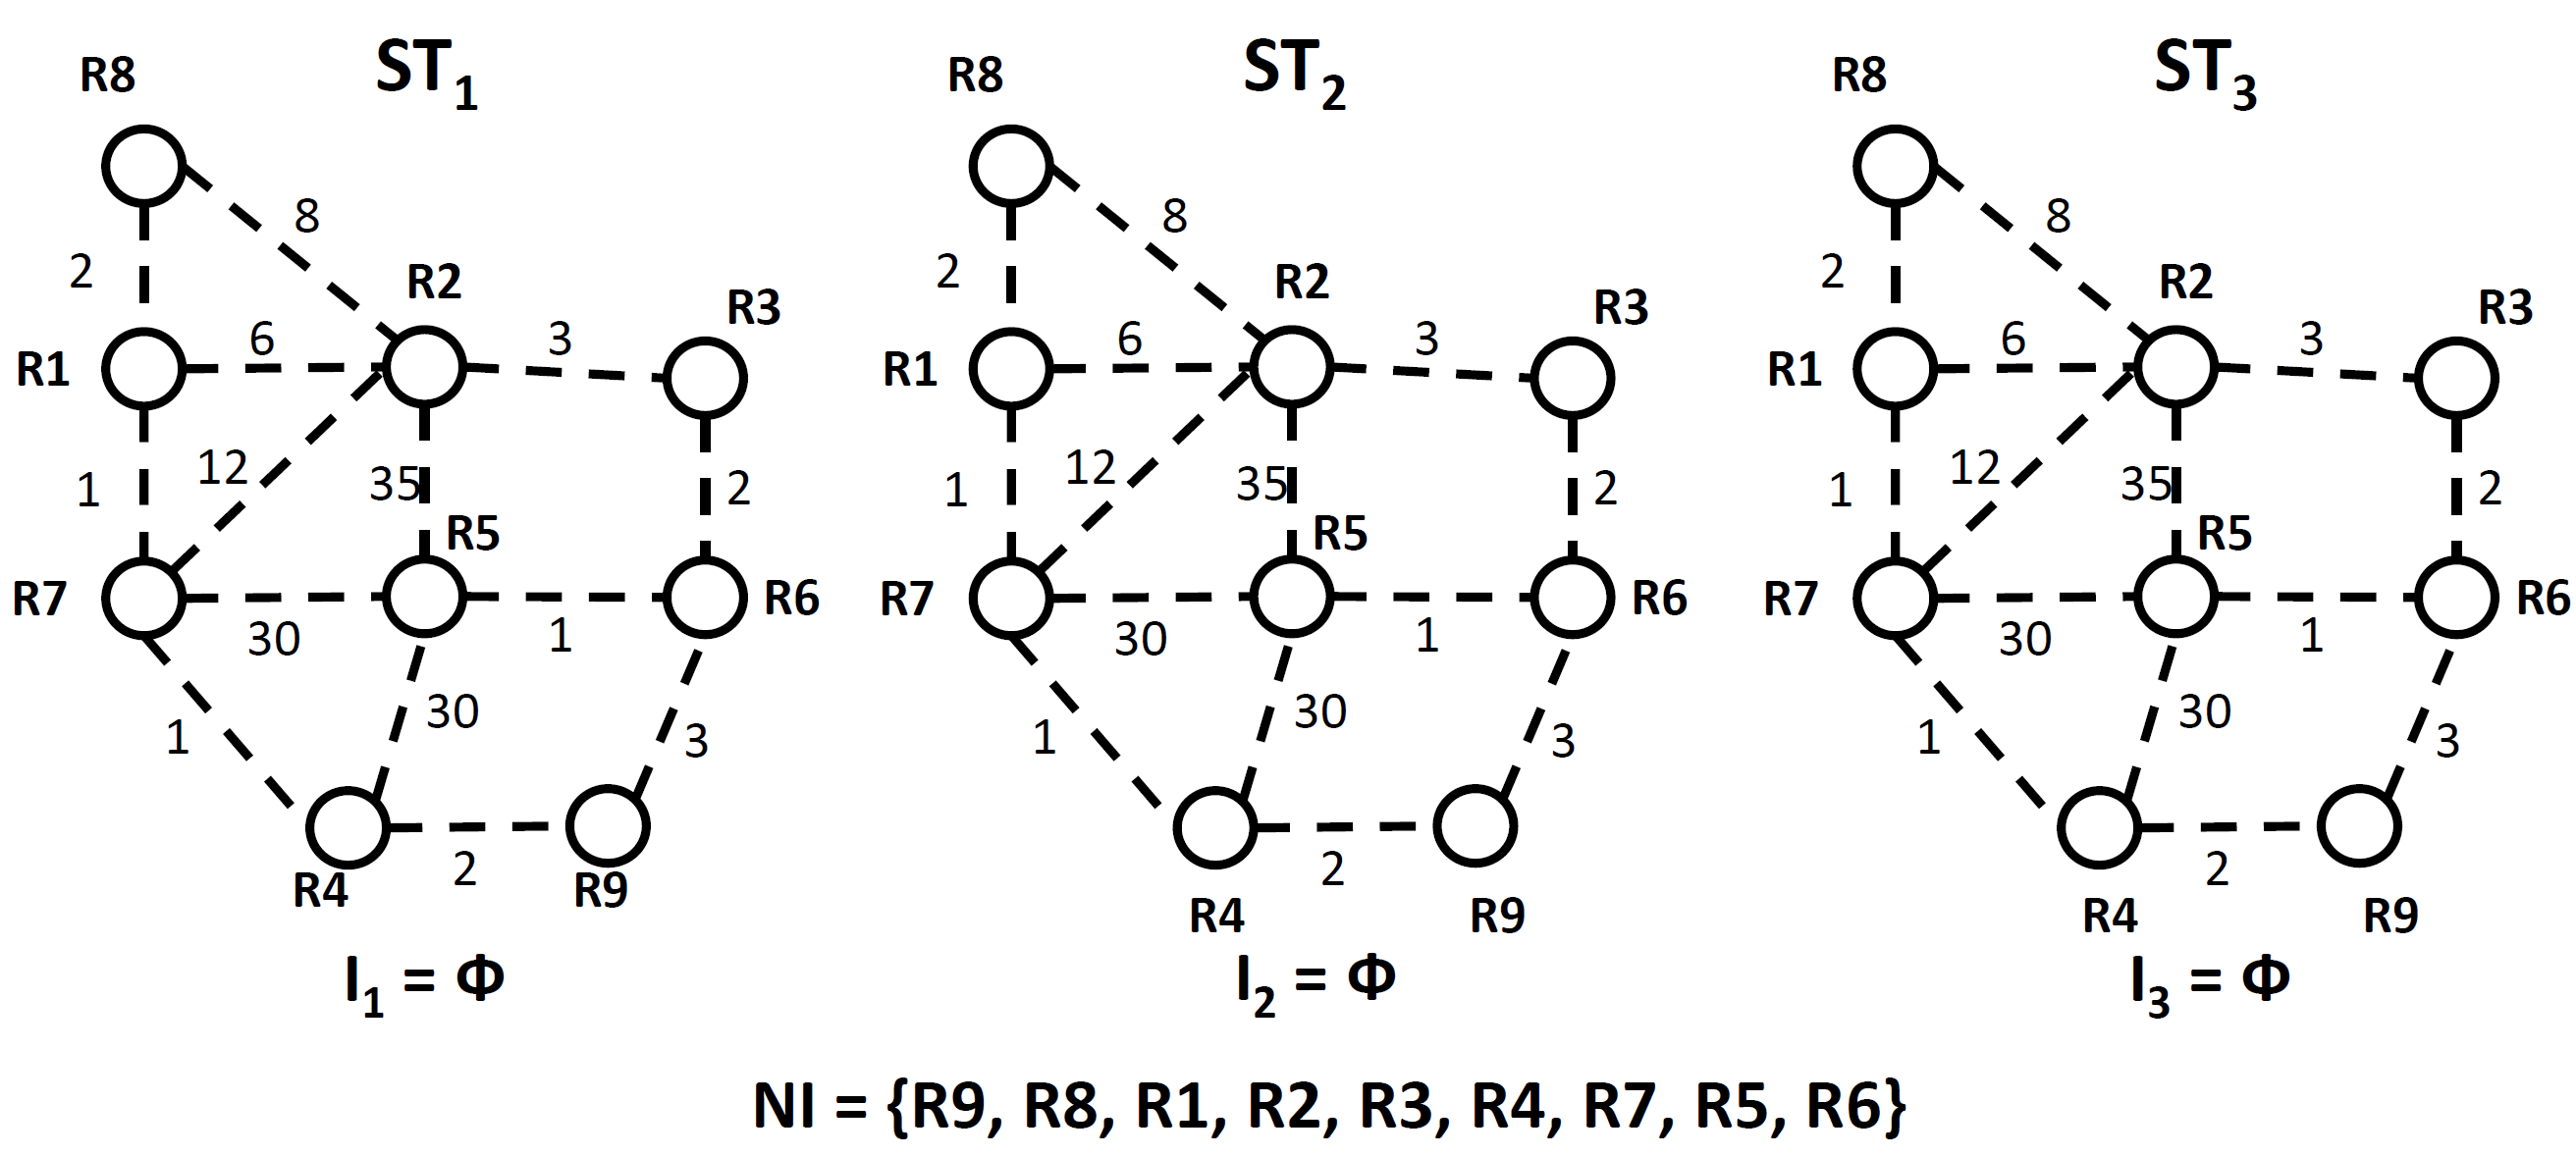
\includegraphics[scale=0.125]{resim.png}
	\caption{Şekil örneği}
	\label{sekil1}
\end{figure}

Lorem ipsum dolor sit amet, consectetur adipiscing elit. Nunc dui ex, varius a mattis sed, vestibulum varius ante. Aliquam maximus ut nisi quis efficitur. Maecenas laoreet nisl vitae tempor aliquam. Donec ac odio suscipit, suscipit magna vitae, pharetra sapien. Cras arcu libero, suscipit ut massa sit amet, tempus euismod augue. Cras eu ligula id nulla luctus facilisis ultrices sit amet lorem. Praesent placerat, lorem eget pharetra dictum, arcu est pharetra ante, vel suscipit mi odio nec sapien. Morbi vehicula elit lacus, sit amet tristique nisi interdum non. Cras convallis neque dui, ut aliquet nulla tempor elementum. Fusce sagittis urna ac mauris mattis condimentum.

Vivamus efficitur a purus eu egestas. Donec feugiat facilisis mauris, at gravida turpis. Mauris quis pellentesque est. Duis in quam sollicitudin massa facilisis fringilla. Proin pulvinar, justo sit amet hendrerit sollicitudin, massa quam euismod felis, porta cursus est tortor nec elit. In mollis nunc eget massa bibendum, vel sagittis enim placerat. Sed luctus porta felis, a faucibus nisi placerat a. Duis velit libero, gravida sed iaculis sodales, consectetur eget metus. Nulla vel magna purus. Sed ligula magna, dignissim sed convallis id, sodales vel libero.


\bibliographystyle{IEEEtran}
\bibliography{references}


% that's all folks
\end{document}